\documentclass{article}

\usepackage{microtype}
\usepackage{graphicx}
\usepackage{subfigure}
\usepackage{booktabs}
\usepackage{kotex} % for korean. 안녕하세요!
\usepackage{amsmath}
\usepackage{amssymb}

\usepackage{hyperref}

\newcommand{\theHalgorithm}{\arabic{algorithm}}

%%%%%%%%%%%%%% wow! this paper is accepted to ICML! HOW? %%%%%%%%%%%%%%
%%%%%%%%%%%%%% wow! this paper is accepted to ICML! HOW? %%%%%%%%%%%%%%
%%%%%%%%%%%%%% wow! this paper is accepted to ICML! HOW? %%%%%%%%%%%%%%
%%%%%%%%%%%%%% wow! this paper is accepted to ICML! HOW? %%%%%%%%%%%%%%
%%%%%%%%%%%%%% wow! this paper is accepted to ICML! HOW? %%%%%%%%%%%%%%
%%%%%%%%%%%%%% wow! this paper is accepted to ICML! HOW? %%%%%%%%%%%%%%
\usepackage[accepted]{icml2019}
%%%%%%%%%%%%%% wow! this paper is accepted to ICML! HOW? %%%%%%%%%%%%%%
%%%%%%%%%%%%%% wow! this paper is accepted to ICML! HOW? %%%%%%%%%%%%%%
%%%%%%%%%%%%%% wow! this paper is accepted to ICML! HOW? %%%%%%%%%%%%%%
%%%%%%%%%%%%%% wow! this paper is accepted to ICML! HOW? %%%%%%%%%%%%%%
%%%%%%%%%%%%%% wow! this paper is accepted to ICML! HOW? %%%%%%%%%%%%%%
%%%%%%%%%%%%%% wow! this paper is accepted to ICML! HOW? %%%%%%%%%%%%%%

\icmltitlerunning{COSE474-2023F: Final Project}

\begin{document}

\twocolumn[
\icmltitle{COSE474-2023F:\\ BERT fine-tuning을 통한 경쟁 프로그래밍 문제 Tag 예측}

\icmlsetsymbol{equal}{*}

\begin{icmlauthorlist}
    2022160012 박세준
\end{icmlauthorlist}

%\icmlaffiliation{ku}{Department of Mathematics, Korea University, Seoul, Korea}

%\icmlcorrespondingauthor{the}{myemail@korea.ac.kr}
%\icmlcorrespondingauthor{Eee Pppp}{ep@eden.co.uk}

\icmlkeywords{NLP, BERT, competitive programming, tag prediction}

\vskip 0.3in
]

%\begin{abstract}
%This document provides a basic paper template and submission guidelines.
%Abstracts must be a single paragraph, ideally between 4--6 sentences long.
%Gross violations will trigger corrections at the camera-ready phase.
%\end{abstract}

\section{Introduction}
경쟁 프로그래밍(Competitive Programming, CP)은 컴퓨터 과학의 비교적 잘 알려진 문제들을 최대한 빠르게 해결하는 것이 
목표인 마인드 스포츠의 일종이다.
경쟁 프로그래밍에 등장하는 문제는 (1)문제 설명, (2)입력/출력 형식 조건, (3)입력/출력 예제, (4)시간, 메모리 제한 등으로 구성되어 있다.
참가자가 문제를 해결하기 위해서는 문제의 시간 및 메모리 제한 안에 동작하고, 주어지는 모든 입력에 대해 옳은 답을 출력하는 프로그램을 제출해야 한다\cite{halim2013competitive}.

경쟁 프로그래밍 문제를 해결하는 과정은 문제를 이해하는 단계, 문제를 해결하기 위한 효율적인 알고리즘을 구상하는 단계, 구상한 알고리즘을 직접 프로그래밍하는 단계로 나눌 수 있다\cite{alphacode}.
일반적인 문제의 경우 그 유형과 난이도가 두 번째 단계인 알고리즘 구상 단계와 밀접한 관련을 갖고 있으므로, '이 문제가 어떤 알고리즘을 통해 해결될 수 있는가'에 대한 정보인 태그(Tag)가 문제 해결의 열쇠가 된다.
따라서 주어진 경쟁 프로그래밍 문제에 대한 태그 예측은 문제를 해결하는 것의 부분 문제로 볼 수 있다.

여러 선행 연구들에서 머신 러닝 기법을 활용한 문제 태그 예측이 시도된 바 있다\cite{iancu2019multilabel, athavale2019}.
일반적으로 태그 예측은 문제의 설명을 분석함으로써 수행된다. 
한 문제는 여러 개의 태그를 가질 수 있으므로, 태그 예측은 문제 본문을 multi-label로 분류하는 문제가 된다.

BERT\cite{devlin2019bert}는 2018년 개발 및 공개된, Transformer에 기반한 여러 자연어 처리 작업에서 SOTA를 달성한 거대 언어 모델이다.
BERT의 학습은 pre-training과 fine-tuning의 두 단계로 나뉘는데, pre-training 단계에서는 대규모 corpus를 학습해 언어의 구조를 학습하고,
fine-tuning에서는 pre-training 단계에서 학습된 결과를 활용하여 모델 출력을 특정 목적에 맞게 미세 조정한다. 사전 학습된 BERT를 활용하면, 
대규모 corpus에서 학습한 언어 구조를 무거운 학습 없이 활용할 수 있다는 강점이 있다.

이 프로젝트는 문제 본문을 활용한 경쟁 프로그래밍 문제의 태그 예측 문제에 BERT를 적용하여 높은 정확도의 태그 예측 모델을 얻는 것을 목표로 두었다.
\section{Method}
 프로젝트의 목적은 자연어 문제 본문을 처리하여 해당 문제의 태그를 예측하는 모델을 학습하는 것이다.
이는 문제 본문의 multi-label 분류 문제로 볼 수 있고, 따라서 프로젝트에서는 
BERT의 768차원 [CLS] 임베딩에 추가로 FC classifier를 덧붙여 fine-tuning을 진행했다.
입력 문제 본문 $stm_i$에 대한 BERT의 768차원 임베딩 $X$에 대하여, 최종 분류 결과 $\hat{Y}_b$는 다음과 같이 쓸 수 있다.
\begin{align}
    \hat{Y} &= \sigma(WX + b)\\
    \hat{Y}_b &= \begin{cases}
        1 & \text{if } \hat{Y} > threshold\\
        0 & \text{otherwise}
    \end{cases}
\end{align}
여기서 $threshold$는 0과 1 사이의 값, activation function $\sigma$는 sigmoid function이고, $(20, 768)$차원 행렬 $W$와 20차원 벡터 $b$는 각각 classifier layer의 weight와 bias에 해당한다.
프로젝트에서 구성한 모델의 전반적인 모식도는 Figure \ref{modelfig}이다.

Multi-label classification을 위해 loss function은 Binary Cross-Entropy Loss로 설정하였으며\cite{Liu2017LearningEB}, 
loss는 참값 $Y$와 $threshold$ 적용 이전의 $\hat{Y}$를 활용해 계산한다.

$threshold$는 각 epoch마다 validation 단계에서 F1-macro score를 최대화하는 값을 grid approximation을 통해 결정하였다.

\begin{figure}[htb!]
    \begin{center}
        \centerline{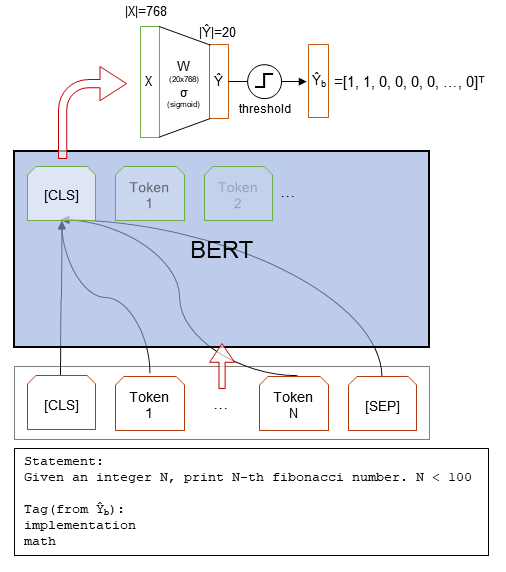
\includegraphics[width=\columnwidth]{fig2.png}}
        \caption{프로젝트 모델}
        \label{modelfig}
    \end{center}
\end{figure}

\section{Experiments}
%\cite{lobanov2023predicting}
\subsection{Datasets}
대부분의 온라인 경쟁 프로그래밍 문제 플랫폼은 문제에 태그를 붙여 관리하고 있다.
\begin{figure}[htb!]
    \begin{center}
        \fbox{
        \begin{minipage}{20em}
            Mathematics, Implementation, Dynamic Programming, Data Structures, 
        Graph Theory, Greedy, String, Bruteforcing, Graph Traversal,
        Sorting, Geometry, Number Theory, Tree, Ad-hoc, Segment Tree,
        Binary Search, Arithmetic, Simulation, Breadth-first Search,
        Constructive, Prefix Sum, Combinatorics, Depth-first Search
        \end{minipage}
        }
        \caption{Online Judge 사이트 \href{https://acmicpc.net}{acmicpc.net}에서 제공하는 상위 23개 태그(문제 수 기준)}
    \end{center}
\end{figure}

이 프로젝트에서는 해외 유명 경쟁 프로그래밍 플랫폼인 \href{https://codeforces.com}{Codeforces}에서 제공하는 문제 중 8234개를 활용하여 문제 설명 - 태그 쌍 데이터를 구성하였다.
이후 문제 수가 가장 많은 상위 20개의 태그를 선택하여 이 태그들만을 학습 대상으로 두었다. 선택된 태그와 태그 별 문항 개수는 Tabel \ref{tags}와 같다.
\begin{table}[htb!]
    \begin{center}
        \begin{tabular}{lc}\toprule
            tag & \# of problems\\\midrule
            implementation & 2219\\
            math & 2027\\
            greedy & 1949\\
            dp & 1672\\
            datastructures & 1288\\
            constructivealgorithms & 1180\\
            bruteforce & 1172\\
            graphs & 901\\
            binarysearch & 785\\
            sortings & 759\\
            dfsandsimilar & 718\\
            trees & 617\\
            strings & 572\\
            numbertheory & 553\\
            conbinatorics & 460\\
            twopointers & 361\\
            bitmasks & 348\\
            geometry & 343\\
            dsu & 247\\
            shortestpaths & 220\\\bottomrule
        \end{tabular}
        \caption{학습 대상으로 설정된 20개의 태그와 각 태그를 갖는 문항의 개수}
        \label{tags}
    \end{center}
\end{table}

각 문제의 태그 참값은 20차원 벡터로 표현되는데, 문제가 $i$번째 태그를 포함하고 있으면 벡터의 $i$번째 요소는 1, 그렇지 않으면 0인 꼴이다.
가령 'implementation, datastructures'태그를 갖는 문제의 경우 태그 정보는 $[1, 0, 0, 0, 1, 0, 0, \ldots, 0]^T$으로 표현된다.
모든 문제 본문은 BERT 토큰화 이전에 lowercase로 변환하였고, 512개를 넘는 토큰으로 변환되는 본문들은 앞 512개의 토큰만을 잘라 사용하였다.

\subsection{Environment}
모든 학습은 Google Colab 환경에서 V100 GPU를 활용하여 이루어졌고, 
코드는 pytorch와 huggingface의 transformers API를 활용하여 작성되었다.

\subsection{Implementation Details}
학습에 사용한 pre-trained BERT 모델은 BERT-Base, Uncased이고, 이는 BERT 원 논문의 \href{https://github.com/google-research/bert}{github repository}에서 다운받을 수 있다.
classifier layer의 dropout 확률은 $0.5$, learning rate는 5e-6으로 설정하였고, 모든 가중치 값은 분포 $Normal(0, 0.02^2)$를 따르도록 초기화되었다.
학습에 사용된 optimizer는 AdamW\cite{loshchilov2019decoupled}이다.

Holdout cross validation을 사용하였으며, Train set과 validation set의 비율은 9:1로 설정하였고, 총 6회의 epoch를 진행했다.

\subsection{Results}
\subsubsection{Quantitative Results}
\begin{table}[htb!]
    \begin{center}
        \begin{tabular}{lccc}\toprule
            Model & F1 Macro & P & R\\\midrule
            TWE+CNN & 0.303 & 0.295 & 0.372 \\
            CNN Ensemble & 0.289 & 0.296 & 0.338 \\
            CNN Ensemble & 0.289 & 0.296 & 0.338 \\\midrule
            BERT(ours) & 0.294 & 0.190 & 0.747\\\bottomrule
        \end{tabular}
        \caption{선행 연구와의 performance 비교(TWE+CNN, CNN Ensemble, GloVe + CNN from \cite{athavale2019})}
        \label{perf}
    \end{center}
\end{table}

\subsubsection{Qualitative Results}

\subsection{Analysis}


\section{Future direction}

\newpage
\bibliography{paper}
\bibliographystyle{icml2019}

\end{document}